\documentclass[twocolumn,10pt,a4paper]{article}
\usepackage[margin=0.75in]{geometry}
\usepackage[utf8]{inputenc}
\usepackage[T1]{fontenc}
\usepackage{lmodern}
\usepackage{microtype}
\usepackage{cite}
\usepackage{url}
\usepackage{hyperref}
\usepackage{xcolor}
\usepackage{enumitem}
\usepackage{tabularx}
\usepackage{booktabs}
\usepackage{graphicx}
\usepackage{tikz}
\usetikzlibrary{positioning,arrows.meta,fit,calc}
\hypersetup{colorlinks=true,citecolor=blue,linkcolor=blue,urlcolor=blue}

\title{Paper 2: Cross-Standards Composition Bridges for Closed-Loop O-RAN Cloud RAN Remediation}

\author{David Kypuros \\
\small Red Hat \\
\small \texttt{dkypuros@redhat.com}}

\date{31 May 2026}

\begin{document}
\maketitle

\begin{abstract}
Paper 2 in this five-paper series describes the cross-standards composition bridge map. An operationally useful closed-loop remediation harness for O-RAN Cloud RAN infrastructure often has to touch contracts from several standards communities: O-RAN Alliance, TM Forum, IEEE, DMTF, and CNCF / Kubernetes SIGs. Published agentic-RAN work commonly starts from one authoritative frame and treats the others as mappings into it, or introduces an additional bridge vocabulary. This paper describes a narrower alternative: each standards body retains authority over its own domain, while the harness composes them at named seam points. We identify six v0 bridges plus one prospective R1 exposure seam, document each with file-level citation metadata in the source repository, and enforce bidirectional standards-lineage traceability through a verify gate a reviewer can run after cloning. We argue that this composition approach is likely to be more durable across spec revisions and easier to discuss in a multivendor ecosystem than a replacement control vocabulary. v0 limits are explicit: local schemas are harness-authored research contracts, several bridges are present at the schema, stub, or fixture-replay layer, and Bridge 7 remains a prospective R1 seam rather than live interop.
\end{abstract}

\section{Introduction}

Cloud RAN Day-2 operations sit at the intersection of several mature but historically separate standards bodies. The O-RAN Alliance defines the SMO-to-O-Cloud interface family \cite{oran_o2_ganp,oran_o2_ims,oran_o2_dms} and the broader architecture \cite{oran_wg1_arch}. TM Forum defines the event-management and intent-management API envelopes \cite{tmf688,tmf921} along with the SID information model \cite{tmf_gb922}. IEEE and ITU-T define the precision timing protocol that gates Cloud RAN service availability \cite{ieee_1588_2019,itu_g82751}. DMTF defines the out-of-band server management interface \cite{dmtf_redfish} that BMCs implement. CNCF and Kubernetes SIGs maintain the CloudEvents envelope \cite{cncf_cloudevents} and the CRD-shaped delivery contracts (MachineConfig \cite{openshift_mco}, KMM Module \cite{kmm_operator}, Metal3 \cite{metal3_project,metal3_bmo}) that actually carry the changes onto a worker node.

An agentic remediation harness has to compose these contracts to produce a credible research loop. Two patterns are common in adjacent work. One begins from a single body, often the SMO frame or a Kubernetes frame, and maps the others into that vocabulary. Another introduces a new bridge layer that asks readers to adopt an additional control vocabulary. Both patterns can be useful, but they make ownership boundaries harder to audit when the underlying specifications revise.

This paper documents a third posture, exercised in the open-source O-RAN Agent Harness referenced by the prior multivendor diagnostic publication \cite{multivendor_blog_2026}. Each body retains authority over its own domain. The harness defines named bridge points where it composes contracts from one body with contracts from another, and each bridge has file-level standards-lineage metadata in the repository. A verify gate validates that the bridge metadata is internally consistent.

Within the shared series spine, Paper 0 frames the work as human-governed intelligence augmentation, Paper 1 describes the O2-IMS-to-operator-CRD architecture, this paper answers how the standards compose, Paper 3 explains why the artifact is falsifiable, and Paper 4 explains the structural communication boundary that contains nondeterministic reasoning. The remainder of this paper is organized as follows. Section \ref{sec:stack} surveys the five standards bodies and their domain authority. Section \ref{sec:bridges} documents six v0 bridges plus one prospective R1 seam. Section \ref{sec:audit} describes the standards-lineage auditing mechanism. Section \ref{sec:compare} compares this approach to ONAP, Nephio, and OSM. Section \ref{sec:conclude} concludes.

\section{The Standards Stack}
\label{sec:stack}

\textbf{O-RAN Alliance.} The O-RAN Architecture Description \cite{oran_wg1_arch} and the Decoupled SMO Architecture technical report \cite{oran_decoupled_smo} define the macro layout. The O2 family \cite{oran_o2_ganp,oran_o2_ims,oran_o2_dms} governs the SMO-to-O-Cloud interfaces. The management-plane family covers O1 \cite{oran_o1} (SMO to managed elements), A1 \cite{oran_a1} (Non-RT RIC to Near-RT RIC), R1 \cite{oran_r1} (SMO-internal service exposure), and E2 \cite{oran_e2} (Near-RT RIC to E2 nodes). The harness targets O2 IMS exclusively for infrastructure remediation; other O-RAN interfaces are referenced as scoping boundaries, not consumed.

\textbf{TM Forum.} TMF688 \cite{tmf688} is the event-management envelope used as the audit sink. TMF921 \cite{tmf921} is the intent-management envelope used for the dual-route notification path. TMF634 \cite{tmf634} (resource inventory) and TMF642 \cite{tmf642} (alarm management) are referenced as background context. The SID information framework \cite{tmf_gb922} grounds the conceptual model. Implementation guides for AIOps \cite{tmf_ig1228}, ODA functional architecture \cite{tmf_ig1190}, and intent management \cite{tmf_ig1253} inform the design without being directly consumed.

\textbf{IEEE and ITU-T.} IEEE 1588-2019 \cite{ieee_1588_2019} defines the Precision Time Protocol state machine (SYNCHRONIZED, HOLDOVER, FREE\_RUNNING, UNCALIBRATED transitions) and the PTP Hardware Clock semantics. The ITU-T G.8275.1 telecom profile \cite{itu_g82751} specifies the full-timing-support deployment posture that Cloud RAN uses.

\textbf{DMTF.} The Redfish specification \cite{dmtf_redfish} governs out-of-band server management. The harness does not consume Redfish directly; Metal3 BMO does, on behalf of the harness, when a firmware push targets a host BMC.

\textbf{CNCF and Kubernetes SIGs.} CloudEvents 1.0 \cite{cncf_cloudevents} is the vendor-neutral event envelope. Three CRD-shaped operators carry the delivery: Machine Config Operator \cite{openshift_mco}, KMM \cite{kmm_operator}, and Metal3 BMO \cite{metal3_bmo}. The MCP specification \cite{mcp_spec} and its Python SDK \cite{mcp_python_sdk} along with the FastMCP framework \cite{fastmcp} provide the internal agent-to-tool scaffolding.

\section{The Composition Bridges}
\label{sec:bridges}

\begin{figure*}[t]
\centering
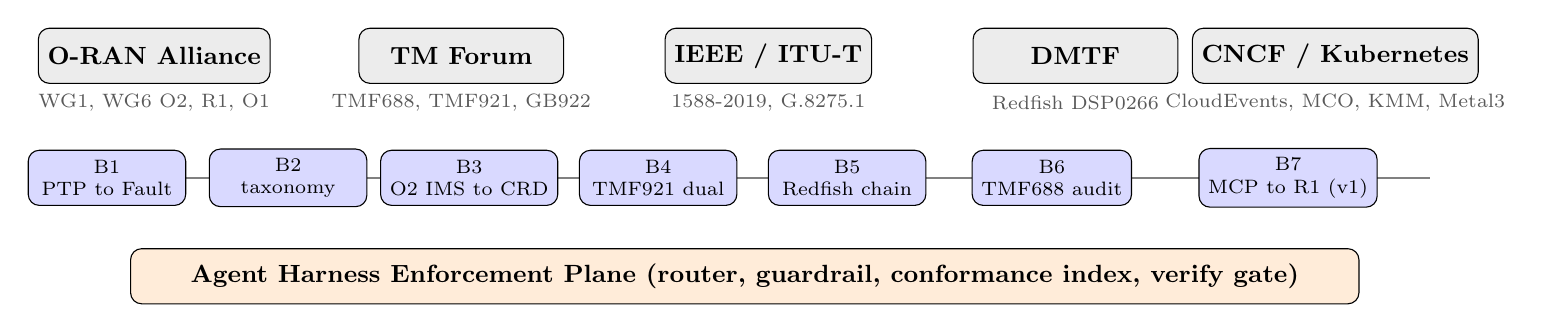
\begin{tikzpicture}[
  body/.style={draw, rounded corners, fill=gray!15, minimum width=2.6cm, minimum height=0.7cm, font=\small\bfseries, align=center},
  spec/.style={draw=none, minimum width=2.6cm, minimum height=0.42cm, font=\scriptsize, align=center, text=black!65},
  bridge/.style={draw, rounded corners, fill=blue!15, minimum width=2.0cm, minimum height=0.7cm, font=\scriptsize, align=center},
  plane/.style={draw, rounded corners, fill=orange!15, minimum width=15.6cm, minimum height=0.7cm, font=\small\bfseries, align=center},
  arr/.style={->, thick, gray!50}
]
\node[body] (oran) at (0, 3.0) {O-RAN Alliance};
\node[body] (tmf)  at (3.9, 3.0) {TM Forum};
\node[body] (ieee) at (7.8, 3.0) {IEEE / ITU-T};
\node[body] (dmtf) at (11.7, 3.0) {DMTF};
\node[body] (k8s)  at (15.0, 3.0) {CNCF / Kubernetes};

\node[spec] at (0, 2.4) {WG1, WG6 O2, R1, O1};
\node[spec] at (3.9, 2.4) {TMF688, TMF921, GB922};
\node[spec] at (7.8, 2.4) {1588-2019, G.8275.1};
\node[spec] at (11.7, 2.4) {Redfish DSP0266};
\node[spec] at (15.0, 2.4) {CloudEvents, MCO, KMM, Metal3};

\draw[thick, gray] (-1.2, 1.45) -- (16.2, 1.45);

\node[bridge] at (-0.6, 1.45) {B1\\ PTP to Fault};
\node[bridge] at (1.7, 1.45)  {B2\\ taxonomy};
\node[bridge] at (4.0, 1.45)  {B3\\ O2 IMS to CRD};
\node[bridge] at (6.4, 1.45)  {B4\\ TMF921 dual};
\node[bridge] at (8.8, 1.45)  {B5\\ Redfish chain};
\node[bridge] at (11.4, 1.45) {B6\\ TMF688 audit};
\node[bridge] at (14.4, 1.45) {B7\\ MCP to R1 (v1)};

\node[plane] at (7.5, 0.2) {Agent Harness Enforcement Plane (router, guardrail, conformance index, verify gate)};

\end{tikzpicture}
\caption{Six v0 contract bridges plus one prospective R1 exposure seam between five standards bodies and the harness enforcement plane. Each bridge corresponds to a subsection of this section. Specific interface references appear under each standards body box. The enforcement plane below the rail is where each bridge becomes machine-checkable through standards-lineage metadata on the relevant authored YAML or JSON artifact.}
\label{fig:bridges}
\end{figure*}

Each bridge below names the from-spec, the to-spec, the seam artifact in the harness, the file anchor where the bridge is implemented, represented, or explicitly marked prospective, and the bibliography references involved. Figure~\ref{fig:bridges} shows the six v0 bridges plus one prospective seam in one view. A reviewer can confirm any single bridge by reading the named files.

\begin{table*}[t]
\centering
\scriptsize
\begin{tabularx}{\textwidth}{p{0.75cm}p{2.2cm}X p{2.5cm}X}
\toprule
Bridge & Bodies composed & Repository anchor & v0 proof level & v1 gap \\
\midrule
B1 & IEEE / ITU-T, CNCF, O-RAN & \texttt{harness/schemas/FaultPayload.json}; \texttt{5G\_O-RAN\_SIM/oam/ptp\_operator\_stub.py}; \texttt{/oran-discover:ptp} & Citation metadata plus inbound fault schema and read-only stub inspection & Live linuxptp to cloud-event-proxy to O-RAN Cloud Notification interop \\
B2 & O-RAN, harness taxonomy & \texttt{harness/taxonomy.yaml}; \texttt{harness/routing-rules/contribution-1-routing-rule.yaml}; \texttt{/oran-discover:taxonomy} & Citation metadata, bidirectional standards-lineage index, deterministic taxonomy lookup & Broader fixture coverage and standards-body review of interpretive subtypes \\
B3 & O-RAN O2 IMS, Kubernetes operators & \texttt{harness/routing-rules/contribution-1-routing-rule.yaml}; \texttt{5G\_O-RAN\_SIM/oam/o2ims\_stub.py}; scenario \texttt{remediation.yaml} fixtures & Real Python call into a shape-correct O2 IMS stub plus fixture replay against CRD-shaped outputs & Live O2 IMS interop and live MCO, KMM, or Metal3 reconciler commits \\
B4 & O-RAN classification, TM Forum TMF921 & \texttt{scenarios/E\_nic\_firmware\_update/companion\_intent.json}; \texttt{scenarios/E\_with\_smo\_reject/companion\_intent.json} & Fixture replay covers accepted and rejected companion-intent outcomes & Live partner-SMO TMF921 exchange and service-window policy integration \\
B5 & DMTF Redfish, Metal3, O-RAN O2 IMS & \texttt{5G\_O-RAN\_SIM/oam/redfish\_bmc\_stub.py}; \texttt{scenarios/E\_nic\_firmware\_update/remediation.yaml}; \texttt{/oran-discover:redfish} & Stub and Metal3 CRD fixture representation only & Live BMC Redfish write path and firmware task verification \\
B6 & TM Forum TMF688, O-RAN, Kubernetes & \texttt{harness/schemas/AuditEvent.json}; scenario \texttt{audit\_event.json} fixtures & Harness-authored audit schema plus end-to-end walker replay on material fields & Formal TMF688 conformance testing and production event-bus wiring \\
B7 & MCP, prospective O-RAN R1 & \texttt{harness/routing-rules/contribution-3-llm-neutrality.yaml}; \texttt{harness/mcp-tool-schemas/*.json} & Declared layering and internal tool-schema metadata only & R1 rApp exposure and live SMO-internal interoperability \\
\bottomrule
\end{tabularx}
\caption{Bridge status at v0. The proof level is intentionally local to the research artifact: metadata traceability, schema shape, stub execution, or fixture replay. It is not a standards-body conformance certificate. Bridge 7 is kept prospective so MCP remains internal scaffolding rather than an O-RAN management-plane claim.}
\label{tab:bridge-status}
\end{table*}

\subsection{Bridge 1: IEEE 1588 / G.8275.1 to O-RAN WG6 Cloud Notifications}

PTP state transitions defined by IEEE 1588 \cite{ieee_1588_2019} under the G.8275.1 profile \cite{itu_g82751} are the raw signal. The linuxptp daemons \cite{linuxptp_ptp4l} expose these states. The cloud-event-proxy sidecar \cite{cloud_event_proxy} translates them into O-RAN.WG6 Cloud Notifications \cite{oran_cloud_notifications} carried over the CNCF CloudEvents 1.0 envelope \cite{cncf_cloudevents}. The harness consumes the resulting envelope as \texttt{FaultPayload}. The bridge chains four standards bodies in one signal path: IEEE / ITU-T timing domain to CNCF event envelope to O-RAN notification contract to the harness's inbound schema. The reviewer-facing inspection surface for this bridge is \texttt{/oran-discover:ptp}, which reads the live PTP wrapper when the lab is running or the committed PTP stub when it is not.

\subsection{Bridge 2: O-RAN WG6 O-Cloud resource model to harness taxonomy}

The harness defines a 20-entry taxonomy of fault classes in \texttt{harness/taxonomy.yaml}. The file opens with an explicit grounding disclaimer: twelve infrastructure subtypes are interpretive mappings within the three normative O-Cloud resource classes from O2 General Aspects and Principles Figure 3.4-1 \cite{oran_o2_ganp} (Physical Resource, Logical Resource, Managed O-Cloud Service), five service-layer subtypes route upward through TMF921, and three ambiguous subtypes require disambiguation before execution. The bridge does not extend the spec; it maps operator-meaningful infrastructure action classes (host configuration, driver swap, node firmware, performance profile, SR-IOV allocation, and related classes) onto pre-existing O-RAN class boundaries while leaving service-layer work outside the infrastructure apply path. The \texttt{/oran-discover:taxonomy} skill is the reviewer-facing view of this mapping.

\subsection{Bridge 3: O-RAN O2 IMS to Kubernetes-native CRDs}

This is the architectural core of the harness. The routing rule at \texttt{harness/routing-rules/contribution-1-routing-rule.yaml} dispatches infrastructure-layer faults through the O2 IMS provisioning surface \cite{oran_o2_ganp,oran_o2_ims} toward Kubernetes-native CRD reconcilers. The reference O2 IMS implementation is Red Hat's O-Cloud Manager \cite{oran_o2ims_ocm}. In v0, a single \texttt{RemediationProposal} exercises a real Python call into a shape-correct O2 IMS stub and carries the resulting \texttt{o2ims\_dispatch} envelope into the audit; committed fixtures represent the downstream CRD-shaped delivery targets. Metal3 HostFirmwareComponents \cite{metal3_bmo} and Machine Config Operator MachineConfig resources \cite{openshift_mco} anchor the named O2-IMS-to-operator-CRD bridge, and Kernel Module Management v1beta1 \cite{kmm_operator} is a co-delivery path within the same bridge for driver-swap action classes. The v0 claim is bridge-shape and fixture replay, not live O2 IMS interop or a live reconciler commit. The \texttt{/oran-discover:metal3} skill exposes the Metal3 side of this bridge as a read-only infrastructure-route check.

\subsection{Bridge 4: O-RAN routing decision to TM Forum intent (TMF921)}

Service-layer faults route up via TMF921 \cite{tmf921}. The harness emits a companion intent and observes the partner SMO's response. The dual-route pattern also fires this bridge for infrastructure-layer faults whose blast radius implies a service window (the canonical case is a node firmware update that forces a host reboot). The bridge crosses the O-RAN resource-layer classification into the TM Forum intent envelope; the audit emits both legs. The \texttt{/oran-discover:smo} skill exposes this service-route state without giving the chat harness authority to emit or change an intent.

\subsection{Bridge 5: DMTF Redfish to Metal3 to O-RAN O2 IMS}

When a firmware push targets a host BMC, Metal3 BMO \cite{metal3_bmo} issues a Redfish UpdateService.SimpleUpdate call \cite{dmtf_redfish}. The harness does not author a Redfish binding; it delegates to Metal3, which in turn responds to the O2 IMS reconciler invocation. The bridge spans three bodies (O-RAN, CNCF / Kubernetes, DMTF) in one delivery path. The honest-scope acknowledgement here: the harness in v0 references the Redfish path through Metal3 stubs but does not exercise it against live BMCs. The \texttt{/oran-discover:redfish} skill is the read-only view of the BMC task side of this chain and should be interpreted together with \texttt{/oran-discover:metal3}.

\subsection{Bridge 6: TM Forum TMF688 as the audit sink}

Every \texttt{RemediationProposal} exits as a TMF688-shaped \texttt{AuditEvent} \cite{tmf688}. The audit carries the proposal, the guardrail result, the sandbox verdict, the O2 IMS dispatch envelope (if the routing target was infrastructure), the companion intent and its dispatch result (if the routing emitted a TMF921 companion), and a seven-field ReversibilityProfile. The bridge here is: an O-RAN-classified action plus a Kubernetes-native payload plus an O-RAN-cited delivery dispatch land inside a TM Forum event envelope as the operator-facing record. TMF688 is the cross-spec lingua franca for the audit row. The \texttt{/oran-discover:guardrail} skill exposes the policy context that determines whether such a proposal can move from audit package to authorized action.

\subsection{Bridge 7: MCP internal scaffolding to O-RAN R1 (prospective)}

The harness's Agentic Gateway exposes vendor-private tooling to agents via MCP \cite{mcp_spec,mcp_python_sdk,fastmcp}. MCP is NOT an O-RAN management plane interface; the layering is declared explicitly in the harness's \texttt{contribution-3-llm-neutrality.yaml}. A future rApp realization that exposes harness capability to other SMO components would expose via R1 \cite{oran_r1}. This is a prospective seam rather than a v0 implemented bridge: the seam is declared in the disclaimer and a v1 rApp deliverable can wire it up without disturbing the v0 internal scaffolding. The \texttt{/oran-discover:plan} skill is not an eighth bridge. It is the pre-flight orchestrator that walks the six v0 bridge-inspection skills in order.

\section{The Standards-Lineage Auditing Mechanism}
\label{sec:audit}

\begin{figure}[t]
\centering
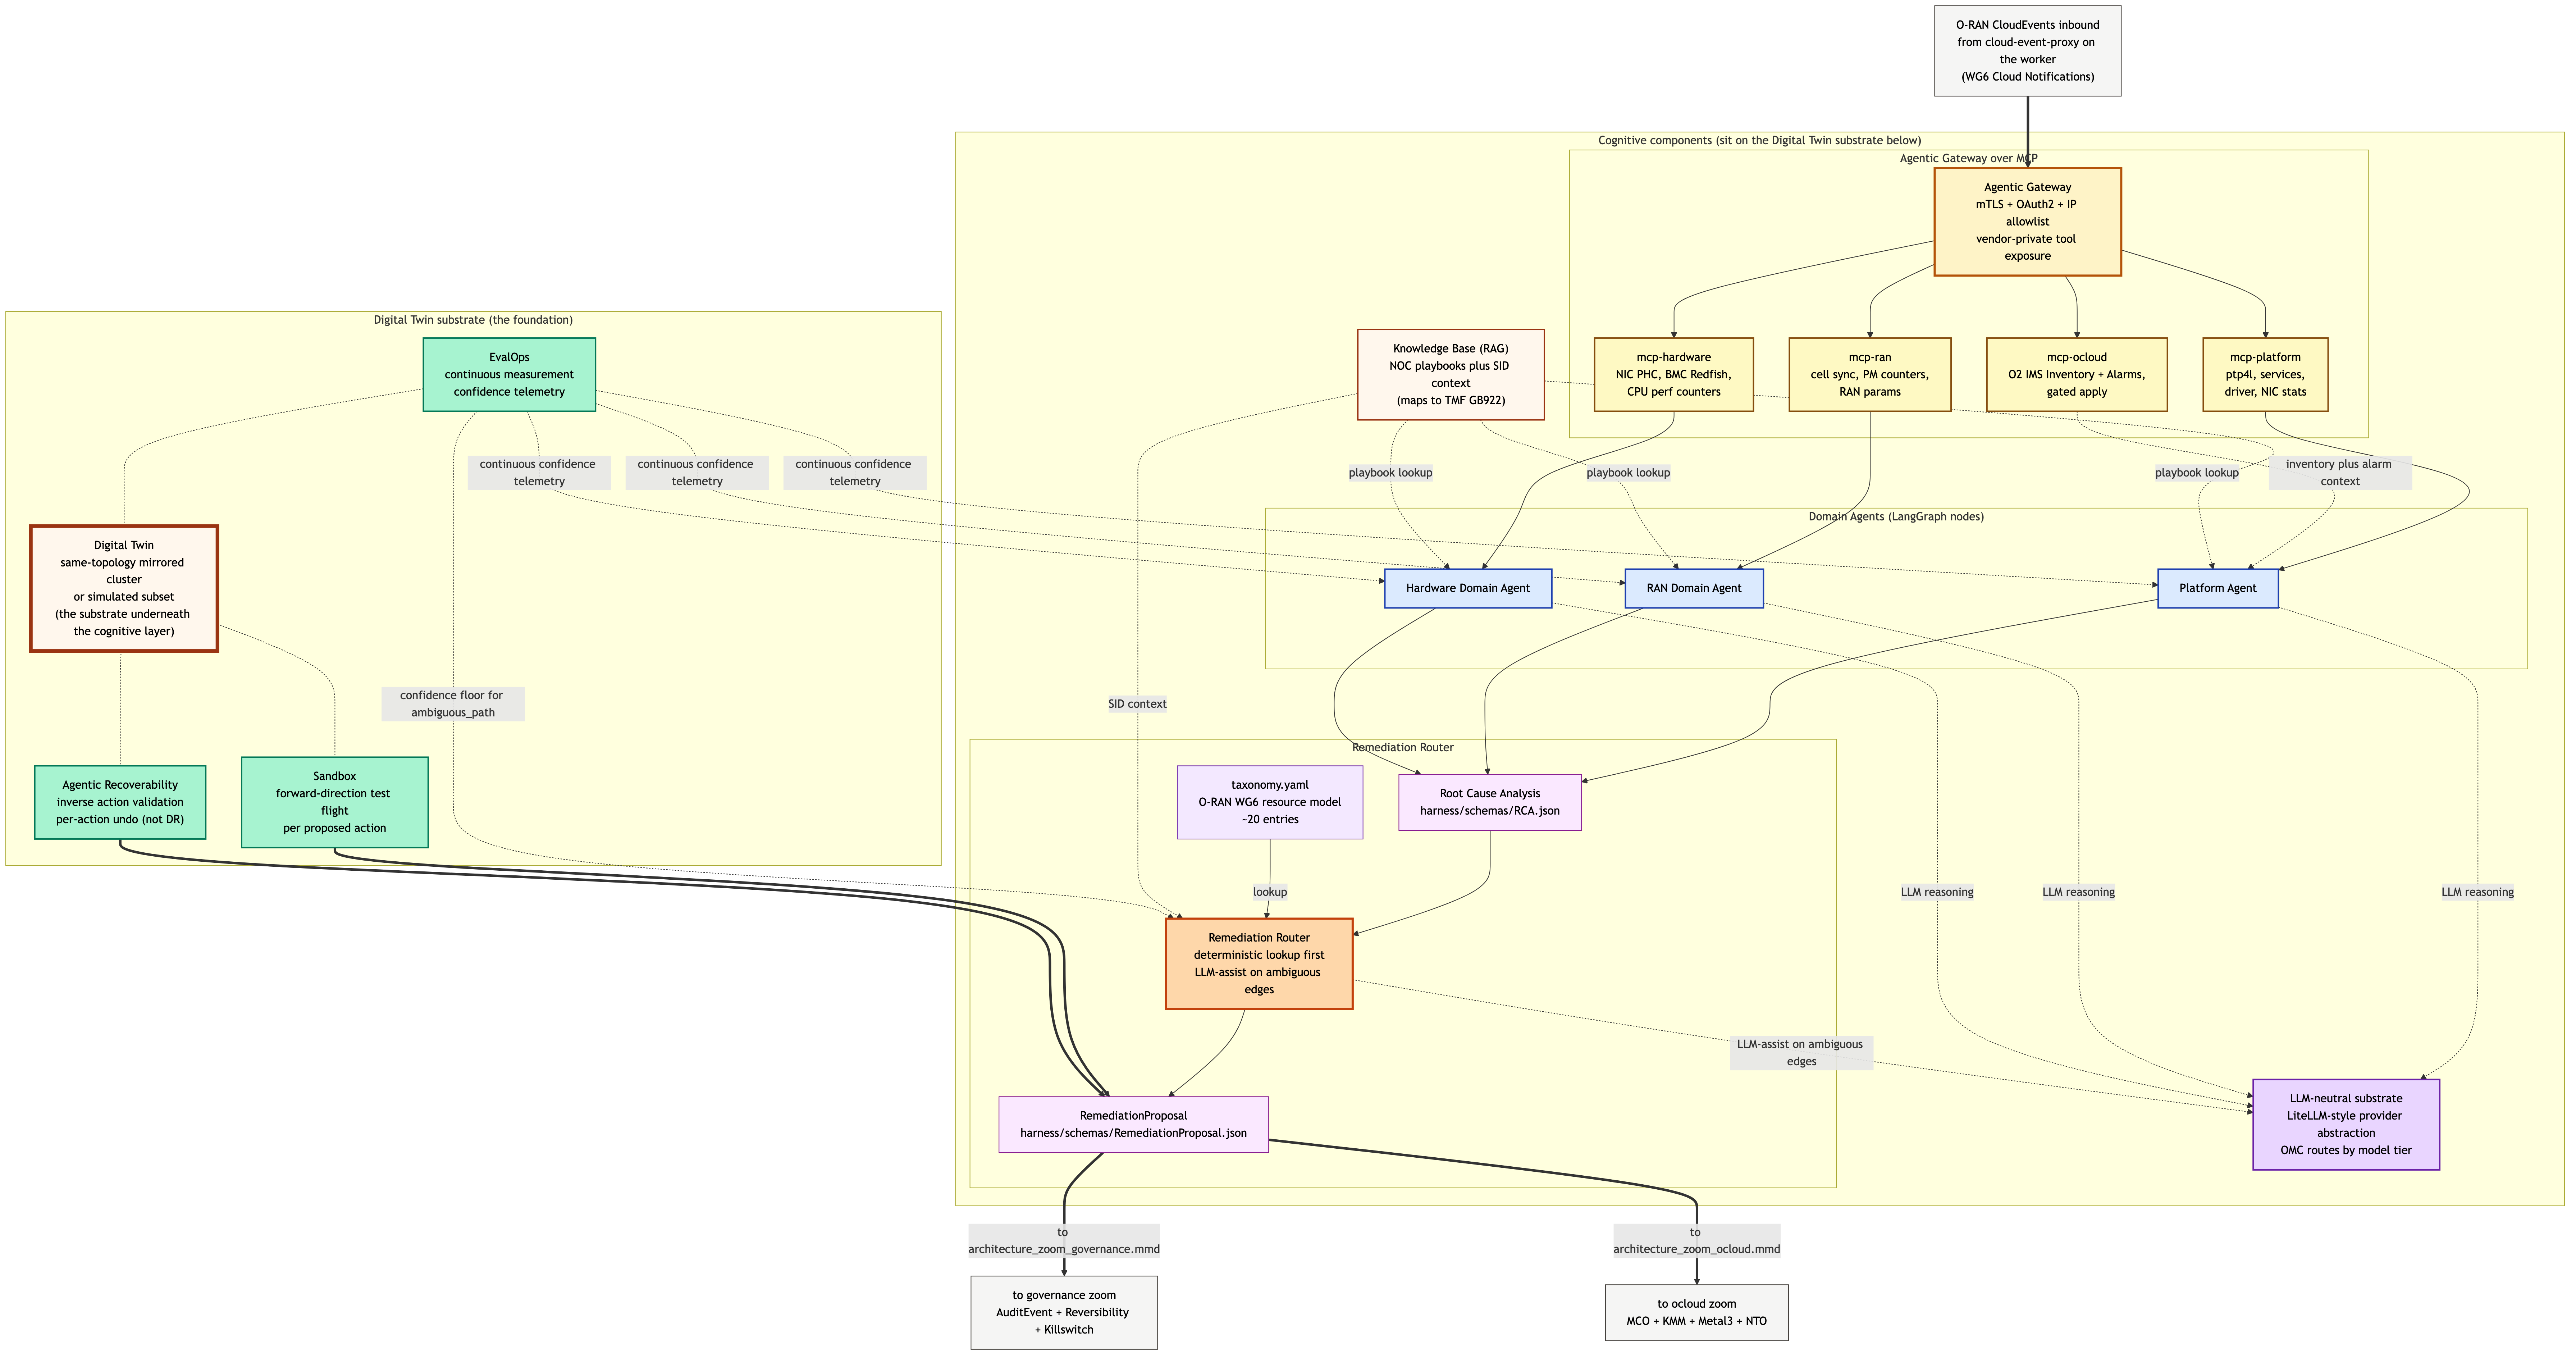
\includegraphics[width=\columnwidth]{../talk/architecture_zoom_cognitive.png}
\caption{Cognitive middle zoom. The Agentic Gateway terminates the CloudEvents stream and presents the MCP server mesh (mcp-platform, mcp-ran, mcp-hardware, mcp-ocloud) to the three domain agents (Platform, RAN, Hardware). The deterministic Router consults the taxonomy and the routing rule. EvalOps, Sandbox, and Agentic Recoverability run as activities on the Digital Twin substrate beneath. Citation-header enforcement and the standards-lineage index sit alongside the Router as machine-checkable contracts.}
\label{fig:cognitive}
\end{figure}

The bridge claims are only useful if a reviewer can confirm them mechanically. The harness ships two enforcement mechanisms.

\textbf{Citation headers on every authored stub.} Every YAML and JSON file under \texttt{harness/} and \texttt{scenarios/} opens with a \texttt{\_conforms\_to} or equivalent block naming the spec, the spec section, and the bibliography references. Failure to add a citation header on a new file fails the verify gate's first check. The mechanism turns documentation into a contract.

\textbf{Bidirectional standards-lineage index.} A file at \texttt{harness/conformance.md} carries a two-column table mapping every authored artifact to its spec lineage. The verify gate's fourth check confirms both directions: no file in the harness tree is missing from the index, and no row in the index points to a file that does not exist. The mechanism prevents the index from rotting silently as the codebase changes. It is a repository traceability check, not a standards-body conformance certification.

A reviewer who disputes any bridge claim in Section \ref{sec:bridges} runs \texttt{python3 scripts/verify.py} from the repository root. Check 1 confirms that every cited file has a citation header. Check 4 confirms that the index is bidirectionally complete. Check 9, when jsonschema is installed, confirms scenario artifacts validate against the harness-authored JSON Schemas. Check 10 replays the walker against every committed scenario fixture and compares output on seven named fields plus the reversibility confidence sub-field. The gate exits non-zero on any failure with a specific row identifying broken bridge metadata, a schema-shape claim, or a fixture-replay claim.

\section{Comparison to Adjacent Projects}
\label{sec:compare}

\textbf{ONAP \cite{onap}.} The Open Network Automation Platform tends to absorb adjacent specs into the ONAP information model and policy framework. This is operationally successful at scale but produces a centralizing posture: ONAP is the authoritative frame, and other specs are mapped into it. The harness pattern described here takes the opposite posture: each spec retains domain authority and the harness composes at named seams. A deployment that runs ONAP for orchestration could compose with this closed-loop harness at the audit and intent bridges (Bridges 4 and 6) without rewriting ONAP's internal model.

\textbf{Nephio \cite{nephio}.} Nephio is cloud-native network automation focused on KRM-based package specialization for orchestration. It does not ship a closed-loop remediation harness. The composition is natural: Nephio delivers the standing topology and post-deployment configuration; the harness handles Day-2 anomalies on top of that topology. Bridges 2, 3, and 6 do not conflict with Nephio's package model; they consume the cluster state Nephio produces.

\textbf{Open Source MANO \cite{osm}.} OSM is mature management and orchestration software. It is spec-aligned with the broader telco automation stack but does not ship a closed-loop remediation substrate with a deterministic taxonomy grounded in O-RAN's resource model. The harness can sit beside OSM in a deployment that wants to use OSM for VNF lifecycle and the harness for Cloud RAN infrastructure remediation.

\textbf{Honest scope.} The composition claim is bridge-by-bridge and v0-bounded, not an interop certification. Six v0 bridges are documented and locally checked at metadata, schema-shape, stub-execution, or fixture-replay level; Bridge 7 is a prospective R1 exposure seam. Several bridges, notably Bridge 5 for live Redfish writes, are represented through stubs or fixtures without live vendor-system interop. The path from "v0 bridges are documented and locally verified" to "v1 bridges are interop-tested against vendor implementations" is future work. The standards-track ask is correspondingly modest: an O-RAN nGRG output that names a Closed-Loop Remediation SMOS as a candidate element of the Decoupled SMO catalogue, and a TMF Implementation Guide discussion of the harness-unique dispatch result extension and seven-field ReversibilityProfile as candidate API additions.

\section{Conclusion}
\label{sec:conclude}

This paper has documented a bridge-based composition architecture that lets a closed-loop Cloud RAN remediation harness touch contracts from five standards bodies (O-RAN Alliance, TM Forum, IEEE, DMTF, CNCF / Kubernetes SIGs) without proposing a replacement standards body. Six v0 bridges plus one prospective R1 seam are documented with file-level standards-lineage anchors. Two enforcement mechanisms (citation headers and a bidirectional standards-lineage index) make the bridges machine-checkable for repository traceability. The verify gate runs in approximately five seconds and exits binary pass/fail for the checks it executes, with full schema validation requiring jsonschema. We hypothesize that the resulting architecture is more durable across spec revisions and politically simpler to land in a multivendor ecosystem than approaches that elevate one body or invent a replacement spec. The v0 limits are declared and the v1 path is named.

\section*{Acknowledgements}

The architecture extends a prior multivendor diagnostic substrate co-authored with S. Kiani Mehr, N. Korati Prasanna, M. Vazquez Cebrian, S. Srikanthan, and P. Venkatesh \cite{multivendor_blog_2026}. The closed-loop extension and the bridge architecture documented in this paper are open-source under Apache-2.0 at \url{https://github.com/dkypuros/oran-agent-harness}.

\bibliographystyle{plain}
\bibliography{refs}

\end{document}
